\documentclass[twoside]{article}

\usepackage{fancyhdr}
\usepackage{parskip}
\usepackage{geometry}
\usepackage{chemfig}
\usepackage{amsmath}
\usepackage{pgfplots}
\usepackage{rotating}
\usepackage{multicol}
\usepackage[style=long3col]{glossaries}
\usepackage{tikz}
\usepackage{setspace}
\usepackage{hyperref}
\usetikzlibrary{arrows,positioning,shapes.geometric}
\usepgfplotslibrary{polar}

\geometry{
    top=20mm,
    bottom=40mm,
    left=20mm,
    right=20mm
}

\pagestyle{fancy}
\fancyhf{}
\renewcommand{\headrulewidth}{0pt}
\fancyfoot[LO]{
    \begin{turn}{180}
        \begin{minipage}{0.4\linewidth}
            \begin{flushright}
                \begin{multicols}{2}
                    \emph{written exclusively under the influence}
                    \begin{turn}{90}
                    \chemfig{[,0.4]*6(([,0.5]=)-([6,0.7]-)-*5(-=-([:60, 0.7]-)-=)--([,0.5]=)-([:150, 0.7]-)-)}
                    \end{turn}
                \end{multicols}
            \end{flushright}
        \end{minipage}
    \end{turn}
}

\fancyfoot[RE]{
    
\includegraphics[width=2cm]{img/qr.png}
}
\fancyfoot[CE,CO]{\thepage}


\title{\underline{A treatise on non-aquatic gastropod Mollusca, a.k.a. \emph{snails}}}
\author{Aayush Bajaj}
\date{\today}

\makenoidxglossaries
\setlength{\glsdescwidth}{0.8\textwidth}
%\renewcommand*{\glsgroupskip}{}

\newglossaryentry{animal}{
    name = {animal},
    sort = {animal},
    description = {Any living thing that is not a plant (basically)}
}
\newglossaryentry{taxonomy}{
    name = {taxonomy},
    sort = {taxonomy},
    description = {The branch of science concerned with classification of living things}
}
\newglossaryentry{phylum}{
    name = {phylum},
    sort = {phylum},
    description = {A level of taxonomic rank}
}
\newglossaryentry{herbivore}{
    name = {herbivore},
    sort = {herbivore},
    description = {An animal that feeds on plants}
}
\newglossaryentry{omnivore}{
    name = {omnivore},
    sort = {omnivore},
    description = {An animal that eats \emph{both} plants and animals}
}
\newglossaryentry{carnivore}{
    name = {carnivore},
    sort = {carnivore},
    description = {An animal that feeds on other animals}
}

\begin{document}

\maketitle % this command implicitly changes the pagestyle to 'title' (duh!)
\thispagestyle{fancy}

\dotfill
\bigbreak

\section*{Definitions}

    \begin{flushright}
    \begin{minipage}{8cm}
        \begin{flushleft} \emph{If you wish to converse with me define your terms.} \end{flushleft}
        \begin{flushright}--- Voltaire\end{flushright}
    \end{minipage}
    \end{flushright}

    Snails are defined as gastropods that have a shell. Gastropods are a \underline{class} of invertebrates which include slugs, squids, octupuses and snails. These gastropods belong to a \textbf{larger} \underline{\gls{phylum}} of \gls{animal}s called \emph{Mollusca}.

\section*{Classifications}
    The gastropod class is the most diverse within the \emph{Molluscs} phylum. Across their aquatic and non-aquatic families gastropods occupy \textbf{every} marine environment from high-energy surge zones to ocean floorbeds.

    Restricting our study to \emph{non-aquatic} gastropods will mean that we encounter almost exclusively the \textbf{prosobranchia} and \textbf{pulmonata} \underline{families}. Interestingly, the pulmonata gastropods respire using lungs whilst the prosobranchia use \emph{gills}. (yes, you can use gills on land as long as they are kept \emph{moist}.)\\

    \begin{tikzpicture}[>=latex']
    \centering
        \tikzset{block/.style= {draw, rectangle, align=center,minimum width=1.7cm,minimum height=1cm}}
        \node [block] (species) {Species};
        \node [block, right =0.6cm of species] (genus) {Genus};
        \node [block, right =0.6cm of genus] (family) {Family};
        \node [block, right =0.6cm of family] (class) {Class};
        \node [block, right =0.6cm of class] (phylum) {Phylum};
        \node [block, right =0.6cm of phylum] (kingdom) {Kingdom};
        \node [block, right =0.6cm of kingdom] (domain) {Domain};
        \node [block, right =0.6cm of domain] (life) {Life};

        \path[draw,->] (species) edge (genus)
                    (genus) edge (family)
                    (family) edge (class)
                    (class) edge (phylum)
                    (phylum) edge (kingdom)
                    (kingdom) edge (domain)
                    (domain) edge (life)
                    ;
        \node [below=1cm, align=flush center,text width=8cm] at (class) { Figure 1: Hierarchy of taxonomic ranks };
    \end{tikzpicture}

\section*{Habitat}
Shelled gastropods can afford to live in more exposed areas than their non-shelled cousins. Gastropods generally prefer to live in damp or wet environments, with the shelled variants preferring forests, wetlands and gardens.


    
\section*{Behaviours}
    Most snails are \gls{herbivore}s, whilst some are \gls{omnivore}s and few are predatory \gls{carnivore}s. The herbivores use their thousands of microscopic pseudo-teeth to file through plants and algae, ripping food into small pieces. Snails eat at night, and some hibernate through the entirety of winter. Snails can hibernate for up to 3 years. They usually live for 2 - 3 years, but some can live for 10.


\newpage
\newgeometry{top=20mm,bottom=25mm,left=20mm,right=20mm}

\begin{multicols}{2}

    \begin{minipage}{0.4\textwidth}
    \section*{Facts}
        \begin{itemize}
            \item Snails are hermaphrodites, they all have pp.
            \item The field of \gls{taxonomy} evolves quickly. Organisms classified as being one type are often later realised to be a subset of another type or dissimilar to the class they were initially categorised in.
            \item The largest land snails grow to 1kg and 38cm in length whilst the largest sea snails can reach 18kg and 90cm in length!
            \item Some snails eat other snails.
            \item Gastropods do not possess the sense of hearing!
            \item Most \emph{terrestrial} (land) snails have shells that are right-handed in their coiling.
            \item During hibernation a snail will seal its shell shut with mucus to stay \emph{moist}.
            \item There is a \underline{genus} of pond snails called \emph{Lymnaea} which only make decisions using two types of neurons: one which decides if it's hungry, and the other deciding if there is food nearby.
        \end{itemize}
        \begin{center}
            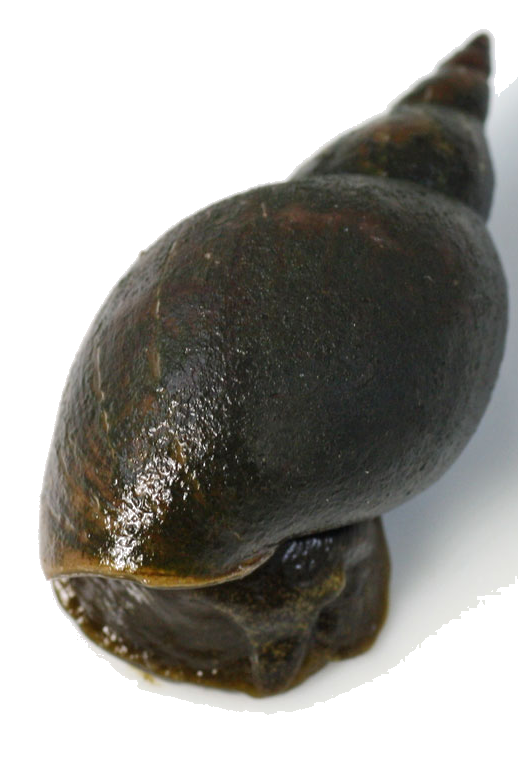
\includegraphics[width=0.3\textwidth]{img/vege.png}\\
            Figure 2: the Lymnaea snail.
        \end{center}
    \end{minipage}

    \begin{flushleft}
    \begin{minipage}{0.5\textwidth}
    \section*{Mathematics}

        Let us briefly consider the length of Jamiroquai the Garden Snail \emph{(a.k.a cornu aspersum)}.
        Approximating the shell function to be defined in polar coordinates as \(r = e^{\frac{-\theta}{10}}\) we may then use \[ l = \int^{\theta_1}_{\theta_0} \sqrt{[f(\theta)]^2 + [f'(\theta)]^2} \, \mathrm{d}\theta .\]

        On

        \begin{center}
            \begin{tikzpicture}[scale = .7]
                \node[inner sep=0pt] (snail) at (0,0)
                    {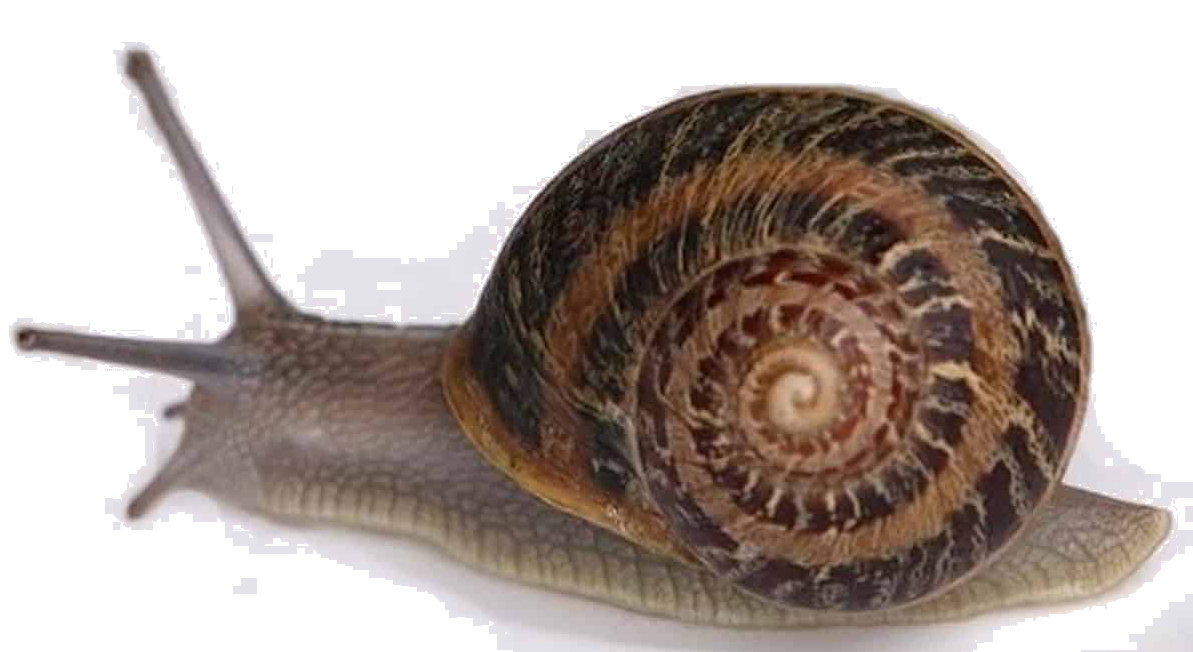
\includegraphics[width=.5\textwidth]{img/snail.png}};
                \node[inner sep=0pt] (spiral) at (-1.9,-2.3) {
                    \begin{polaraxis}[axis lines=none, scale = .4]
                        \addplot[domain=0:1260, samples=1000, line width = 1mm]{e^0.1*x};
                    \end{polaraxis}
                    };
                    \node [below=1cm, align=flush center,text width=8cm] at (spiral) { Figure 3: Jamiroquai };
            \end{tikzpicture}
        \end{center}

        Such that the unravelled length of Mr Aspersum's shell becomes 
        \begin{align*}
            l &= \int^{\theta_1}_{0} \sqrt{(e^{-\frac{\theta}{10}})^2 + (-\frac{1}{10}e^{-\frac{\theta}{10}})^2}\mathrm{d}\theta\\
            &= \int^{\theta_1}_{0} \sqrt{(1+\frac{1}{100})e^{-\frac{2\theta}{10}}} \mathrm{d}\theta\\
            &= \frac{\sqrt{101}}{10} \int^{\theta_1}_0 e^{-\frac{\theta}{10}}\mathrm{d}\theta\\
            &= \sqrt{101}(1 - e^{-\frac{\theta_1}{10}}).\\
            &= \sqrt{101} \text{ (as \(\theta_1 \rightarrow \infty\)).}
        \end{align*}

    \end{minipage}
    \end{flushleft}

\end{multicols}

\setlength{\parskip}{0pt}

\printnoidxglossary[style=listdotted]

\begin{thebibliography}{8}
    \bibitem{bj1} Brian. J. Smith, \emph{Identification keys to the families and genera of bivalve and gastropod molluscs found in Australian inland waters}, 1996
    \bibitem{bj2} Brian. J. Smith, \emph{Non-marine Mollusca}, 1992
    \bibitem{wiki} Wikipedia, \emph{Online: \url{https://en.wikipedia.org/wiki/Snail}}

\end{thebibliography}


\end{document}
